% Options for packages loaded elsewhere
\PassOptionsToPackage{unicode}{hyperref}
\PassOptionsToPackage{hyphens}{url}
\PassOptionsToPackage{dvipsnames,svgnames,x11names}{xcolor}
%
\documentclass[
  letterpaper,
  DIV=11,
  numbers=noendperiod]{scrartcl}

\usepackage{amsmath,amssymb}
\usepackage{lmodern}
\usepackage{iftex}
\ifPDFTeX
  \usepackage[T1]{fontenc}
  \usepackage[utf8]{inputenc}
  \usepackage{textcomp} % provide euro and other symbols
\else % if luatex or xetex
  \usepackage{unicode-math}
  \defaultfontfeatures{Scale=MatchLowercase}
  \defaultfontfeatures[\rmfamily]{Ligatures=TeX,Scale=1}
\fi
% Use upquote if available, for straight quotes in verbatim environments
\IfFileExists{upquote.sty}{\usepackage{upquote}}{}
\IfFileExists{microtype.sty}{% use microtype if available
  \usepackage[]{microtype}
  \UseMicrotypeSet[protrusion]{basicmath} % disable protrusion for tt fonts
}{}
\makeatletter
\@ifundefined{KOMAClassName}{% if non-KOMA class
  \IfFileExists{parskip.sty}{%
    \usepackage{parskip}
  }{% else
    \setlength{\parindent}{0pt}
    \setlength{\parskip}{6pt plus 2pt minus 1pt}}
}{% if KOMA class
  \KOMAoptions{parskip=half}}
\makeatother
\usepackage{xcolor}
\setlength{\emergencystretch}{3em} % prevent overfull lines
\setcounter{secnumdepth}{-\maxdimen} % remove section numbering
% Make \paragraph and \subparagraph free-standing
\ifx\paragraph\undefined\else
  \let\oldparagraph\paragraph
  \renewcommand{\paragraph}[1]{\oldparagraph{#1}\mbox{}}
\fi
\ifx\subparagraph\undefined\else
  \let\oldsubparagraph\subparagraph
  \renewcommand{\subparagraph}[1]{\oldsubparagraph{#1}\mbox{}}
\fi

\usepackage{color}
\usepackage{fancyvrb}
\newcommand{\VerbBar}{|}
\newcommand{\VERB}{\Verb[commandchars=\\\{\}]}
\DefineVerbatimEnvironment{Highlighting}{Verbatim}{commandchars=\\\{\}}
% Add ',fontsize=\small' for more characters per line
\usepackage{framed}
\definecolor{shadecolor}{RGB}{241,243,245}
\newenvironment{Shaded}{\begin{snugshade}}{\end{snugshade}}
\newcommand{\AlertTok}[1]{\textcolor[rgb]{0.68,0.00,0.00}{#1}}
\newcommand{\AnnotationTok}[1]{\textcolor[rgb]{0.37,0.37,0.37}{#1}}
\newcommand{\AttributeTok}[1]{\textcolor[rgb]{0.40,0.45,0.13}{#1}}
\newcommand{\BaseNTok}[1]{\textcolor[rgb]{0.68,0.00,0.00}{#1}}
\newcommand{\BuiltInTok}[1]{\textcolor[rgb]{0.00,0.23,0.31}{#1}}
\newcommand{\CharTok}[1]{\textcolor[rgb]{0.13,0.47,0.30}{#1}}
\newcommand{\CommentTok}[1]{\textcolor[rgb]{0.37,0.37,0.37}{#1}}
\newcommand{\CommentVarTok}[1]{\textcolor[rgb]{0.37,0.37,0.37}{\textit{#1}}}
\newcommand{\ConstantTok}[1]{\textcolor[rgb]{0.56,0.35,0.01}{#1}}
\newcommand{\ControlFlowTok}[1]{\textcolor[rgb]{0.00,0.23,0.31}{#1}}
\newcommand{\DataTypeTok}[1]{\textcolor[rgb]{0.68,0.00,0.00}{#1}}
\newcommand{\DecValTok}[1]{\textcolor[rgb]{0.68,0.00,0.00}{#1}}
\newcommand{\DocumentationTok}[1]{\textcolor[rgb]{0.37,0.37,0.37}{\textit{#1}}}
\newcommand{\ErrorTok}[1]{\textcolor[rgb]{0.68,0.00,0.00}{#1}}
\newcommand{\ExtensionTok}[1]{\textcolor[rgb]{0.00,0.23,0.31}{#1}}
\newcommand{\FloatTok}[1]{\textcolor[rgb]{0.68,0.00,0.00}{#1}}
\newcommand{\FunctionTok}[1]{\textcolor[rgb]{0.28,0.35,0.67}{#1}}
\newcommand{\ImportTok}[1]{\textcolor[rgb]{0.00,0.46,0.62}{#1}}
\newcommand{\InformationTok}[1]{\textcolor[rgb]{0.37,0.37,0.37}{#1}}
\newcommand{\KeywordTok}[1]{\textcolor[rgb]{0.00,0.23,0.31}{#1}}
\newcommand{\NormalTok}[1]{\textcolor[rgb]{0.00,0.23,0.31}{#1}}
\newcommand{\OperatorTok}[1]{\textcolor[rgb]{0.37,0.37,0.37}{#1}}
\newcommand{\OtherTok}[1]{\textcolor[rgb]{0.00,0.23,0.31}{#1}}
\newcommand{\PreprocessorTok}[1]{\textcolor[rgb]{0.68,0.00,0.00}{#1}}
\newcommand{\RegionMarkerTok}[1]{\textcolor[rgb]{0.00,0.23,0.31}{#1}}
\newcommand{\SpecialCharTok}[1]{\textcolor[rgb]{0.37,0.37,0.37}{#1}}
\newcommand{\SpecialStringTok}[1]{\textcolor[rgb]{0.13,0.47,0.30}{#1}}
\newcommand{\StringTok}[1]{\textcolor[rgb]{0.13,0.47,0.30}{#1}}
\newcommand{\VariableTok}[1]{\textcolor[rgb]{0.07,0.07,0.07}{#1}}
\newcommand{\VerbatimStringTok}[1]{\textcolor[rgb]{0.13,0.47,0.30}{#1}}
\newcommand{\WarningTok}[1]{\textcolor[rgb]{0.37,0.37,0.37}{\textit{#1}}}

\providecommand{\tightlist}{%
  \setlength{\itemsep}{0pt}\setlength{\parskip}{0pt}}\usepackage{longtable,booktabs,array}
\usepackage{calc} % for calculating minipage widths
% Correct order of tables after \paragraph or \subparagraph
\usepackage{etoolbox}
\makeatletter
\patchcmd\longtable{\par}{\if@noskipsec\mbox{}\fi\par}{}{}
\makeatother
% Allow footnotes in longtable head/foot
\IfFileExists{footnotehyper.sty}{\usepackage{footnotehyper}}{\usepackage{footnote}}
\makesavenoteenv{longtable}
\usepackage{graphicx}
\makeatletter
\def\maxwidth{\ifdim\Gin@nat@width>\linewidth\linewidth\else\Gin@nat@width\fi}
\def\maxheight{\ifdim\Gin@nat@height>\textheight\textheight\else\Gin@nat@height\fi}
\makeatother
% Scale images if necessary, so that they will not overflow the page
% margins by default, and it is still possible to overwrite the defaults
% using explicit options in \includegraphics[width, height, ...]{}
\setkeys{Gin}{width=\maxwidth,height=\maxheight,keepaspectratio}
% Set default figure placement to htbp
\makeatletter
\def\fps@figure{htbp}
\makeatother

\usepackage{booktabs}
\usepackage{longtable}
\usepackage{array}
\usepackage{multirow}
\usepackage{wrapfig}
\usepackage{float}
\usepackage{colortbl}
\usepackage{pdflscape}
\usepackage{tabu}
\usepackage{threeparttable}
\usepackage{threeparttablex}
\usepackage[normalem]{ulem}
\usepackage{makecell}
\usepackage{xcolor}
\usepackage{siunitx}
\newcolumntype{d}{S[input-symbols = ()]}
\KOMAoption{captions}{tableheading}
\makeatletter
\makeatother
\makeatletter
\makeatother
\makeatletter
\@ifpackageloaded{caption}{}{\usepackage{caption}}
\AtBeginDocument{%
\ifdefined\contentsname
  \renewcommand*\contentsname{Table of contents}
\else
  \newcommand\contentsname{Table of contents}
\fi
\ifdefined\listfigurename
  \renewcommand*\listfigurename{List of Figures}
\else
  \newcommand\listfigurename{List of Figures}
\fi
\ifdefined\listtablename
  \renewcommand*\listtablename{List of Tables}
\else
  \newcommand\listtablename{List of Tables}
\fi
\ifdefined\figurename
  \renewcommand*\figurename{Figure}
\else
  \newcommand\figurename{Figure}
\fi
\ifdefined\tablename
  \renewcommand*\tablename{Table}
\else
  \newcommand\tablename{Table}
\fi
}
\@ifpackageloaded{float}{}{\usepackage{float}}
\floatstyle{ruled}
\@ifundefined{c@chapter}{\newfloat{codelisting}{h}{lop}}{\newfloat{codelisting}{h}{lop}[chapter]}
\floatname{codelisting}{Listing}
\newcommand*\listoflistings{\listof{codelisting}{List of Listings}}
\makeatother
\makeatletter
\@ifpackageloaded{caption}{}{\usepackage{caption}}
\@ifpackageloaded{subcaption}{}{\usepackage{subcaption}}
\makeatother
\makeatletter
\@ifpackageloaded{tcolorbox}{}{\usepackage[many]{tcolorbox}}
\makeatother
\makeatletter
\@ifundefined{shadecolor}{\definecolor{shadecolor}{rgb}{.97, .97, .97}}
\makeatother
\makeatletter
\makeatother
\ifLuaTeX
  \usepackage{selnolig}  % disable illegal ligatures
\fi
\IfFileExists{bookmark.sty}{\usepackage{bookmark}}{\usepackage{hyperref}}
\IfFileExists{xurl.sty}{\usepackage{xurl}}{} % add URL line breaks if available
\urlstyle{same} % disable monospaced font for URLs
\hypersetup{
  pdftitle={Difference-in-differences},
  colorlinks=true,
  linkcolor={blue},
  filecolor={Maroon},
  citecolor={Blue},
  urlcolor={Blue},
  pdfcreator={LaTeX via pandoc}}

\title{Difference-in-differences}
\author{}
\date{}

\begin{document}
\maketitle
\ifdefined\Shaded\renewenvironment{Shaded}{\begin{tcolorbox}[enhanced, frame hidden, interior hidden, boxrule=0pt, borderline west={3pt}{0pt}{shadecolor}, sharp corners, breakable]}{\end{tcolorbox}}\fi

If you want to follow along with this example, you can download the data
below:

\begin{itemize}
\tightlist
\item
  \href{/files/data/package_data/injury.csv}{ \texttt{injury.csv}}
\end{itemize}

\hypertarget{program-background}{%
\subsection{Program background}\label{program-background}}

In 1980, Kentucky raised its cap on weekly earnings that were covered by
worker's compensation. We want to know if this new policy caused workers
to spend more time unemployed. If benefits are not generous enough, then
workers could sue companies for on-the-job injuries, while overly
generous benefits could cause moral hazard issues and induce workers to
be more reckless on the job, or to claim that off-the-job injuries were
incurred while at work.

The main outcome variable we care about is \texttt{log\_duration} (in
the original data as \texttt{ldurat}, but we rename it to be more human
readable), or the logged duration (in weeks) of worker's compensation
benefits. We log it because the variable is fairly skewed---most people
are unemployed for a few weeks, with some unemployed for a long time.
The policy was designed so that the cap increase did not affect
low-earnings workers, but did affect high-earnings workers, so we use
low-earnings workers as our control group and high-earnings workers as
our treatment group.

The data is included in the \textbf{wooldridge} R package as the
\texttt{injury} dataset, and if you install the package, load it with
\texttt{library(wooldridge)}, and run \texttt{?injury} in the console,
you can see complete details about what's in it. To give you more
practice with loading data from external files, I exported the injury
data as a CSV file (using \texttt{write\_csv(injury,\ "injury.csv")})
and included it here.

These are the main columns we'll worry about for now:

\begin{itemize}
\tightlist
\item
  \texttt{durat} (which we'll rename to \texttt{duration}): Duration of
  unemployment benefits, measured in weeks
\item
  \texttt{ldurat} (which we'll rename to \texttt{log\_duration}): Logged
  version of \texttt{durat} (\texttt{log(durat)})
\item
  \texttt{after\_1980} (which we'll rename to \texttt{after\_1980}):
  Indicator variable marking if the observation happened before (0) or
  after (1) the policy change in 1980. This is our \textbf{time} (or
  \emph{before/after} variable)
\item
  \texttt{highearn}: Indicator variable marking if the observation is a
  low (0) or high (1) earner. This is our \textbf{group} (or
  \emph{treatment/control}) variable
\end{itemize}

\hypertarget{load-and-clean-data}{%
\subsection{Load and clean data}\label{load-and-clean-data}}

First, let's download the dataset (if you haven't already), put in a
folder named \texttt{data}, and load it:

\begin{itemize}
\tightlist
\item
  \href{/files/data/package_data/injury.csv}{ \texttt{injury.csv}}
\end{itemize}

\begin{Shaded}
\begin{Highlighting}[]
\FunctionTok{library}\NormalTok{(tidyverse)  }\CommentTok{\# ggplot(), \%\textgreater{}\%, mutate(), and friends}
\FunctionTok{library}\NormalTok{(broom)  }\CommentTok{\# Convert models to data frames}
\FunctionTok{library}\NormalTok{(scales)  }\CommentTok{\# Format numbers with functions like comma(), percent(), and dollar()}
\FunctionTok{library}\NormalTok{(modelsummary)  }\CommentTok{\# Create side{-}by{-}side regression tables}
\FunctionTok{library}\NormalTok{(readr)}
\end{Highlighting}
\end{Shaded}

\begin{Shaded}
\begin{Highlighting}[]
\CommentTok{\# Load the data.}
\CommentTok{\# It\textquotesingle{}d be a good idea to click on the "injury\_raw" object in the Environment}
\CommentTok{\# panel in RStudio to see what the data looks like after you load it}
\NormalTok{injury\_raw }\OtherTok{\textless{}{-}} \FunctionTok{read\_csv}\NormalTok{(}\StringTok{"injury.csv"}\NormalTok{)}
\end{Highlighting}
\end{Shaded}

Next we'll clean up the \texttt{injury\_raw} data a little to limit the
data to just observations from Kentucky. we'll also rename some
awkwardly-named columns:

\begin{Shaded}
\begin{Highlighting}[]
\NormalTok{injury }\OtherTok{\textless{}{-}}\NormalTok{ injury\_raw }\SpecialCharTok{\%\textgreater{}\%}
  \FunctionTok{filter}\NormalTok{(ky }\SpecialCharTok{==} \DecValTok{1}\NormalTok{) }\SpecialCharTok{\%\textgreater{}\%}
  \CommentTok{\# The syntax for rename is \textasciigrave{}new\_name = original\_name\textasciigrave{}}
  \FunctionTok{rename}\NormalTok{(}\AttributeTok{duration =}\NormalTok{ durat, }\AttributeTok{log\_duration =}\NormalTok{ ldurat,}
         \AttributeTok{after\_1980 =}\NormalTok{ afchnge)}
\end{Highlighting}
\end{Shaded}

\hypertarget{exploratory-data-analysis}{%
\subsection{Exploratory data analysis}\label{exploratory-data-analysis}}

First we can look at the distribution of unemployment benefits across
high and low earners (our control and treatment groups):

\begin{Shaded}
\begin{Highlighting}[]
\FunctionTok{ggplot}\NormalTok{(}\AttributeTok{data =}\NormalTok{ injury, }\FunctionTok{aes}\NormalTok{(}\AttributeTok{x =}\NormalTok{ duration)) }\SpecialCharTok{+}
  \CommentTok{\# binwidth = 8 makes each column represent 2 months (8 weeks)}
  \CommentTok{\# boundary = 0 make it so the 0{-}8 bar starts at 0 and isn\textquotesingle{}t {-}4 to 4}
  \FunctionTok{geom\_histogram}\NormalTok{(}\AttributeTok{binwidth =} \DecValTok{8}\NormalTok{, }\AttributeTok{color =} \StringTok{"white"}\NormalTok{, }\AttributeTok{boundary =} \DecValTok{0}\NormalTok{) }\SpecialCharTok{+}
  \FunctionTok{facet\_wrap}\NormalTok{(}\FunctionTok{vars}\NormalTok{(highearn))}
\end{Highlighting}
\end{Shaded}

\begin{figure}[H]

{\centering 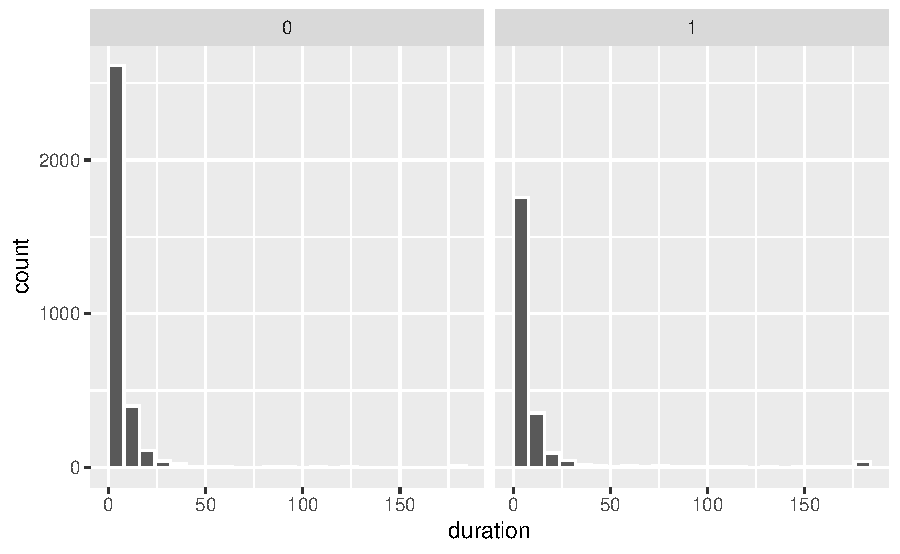
\includegraphics[width=0.75\textwidth,height=\textheight]{DD_wooldridge_injury_files/figure-pdf/duration-histogram-1.pdf}

}

\end{figure}

The distribution is really skewed, with most people in both groups
getting between 0-8 weeks of benefits (and a handful with more than 180
weeks! that's 3.5 years!)

If we use the log of duration, we can get a less skewed distribution
that works better with regression models:

\begin{Shaded}
\begin{Highlighting}[]
\FunctionTok{ggplot}\NormalTok{(}\AttributeTok{data =}\NormalTok{ injury, }\AttributeTok{mapping =} \FunctionTok{aes}\NormalTok{(}\AttributeTok{x =}\NormalTok{ log\_duration)) }\SpecialCharTok{+}
  \FunctionTok{geom\_histogram}\NormalTok{(}\AttributeTok{binwidth =} \FloatTok{0.5}\NormalTok{, }\AttributeTok{color =} \StringTok{"white"}\NormalTok{, }\AttributeTok{boundary =} \DecValTok{0}\NormalTok{) }\SpecialCharTok{+}
  \CommentTok{\# Uncomment this line if you want to exponentiate the logged values on the}
  \CommentTok{\# x{-}axis. Instead of showing 1, 2, 3, etc., it\textquotesingle{}ll show e\^{}1, e\^{}2, e\^{}3, etc. and}
  \CommentTok{\# make the labels more human readable}
  \CommentTok{\# scale\_x\_continuous(labels = trans\_format("exp", format = round)) +}
  \FunctionTok{facet\_wrap}\NormalTok{(}\FunctionTok{vars}\NormalTok{(highearn))}
\end{Highlighting}
\end{Shaded}

\begin{figure}[H]

{\centering 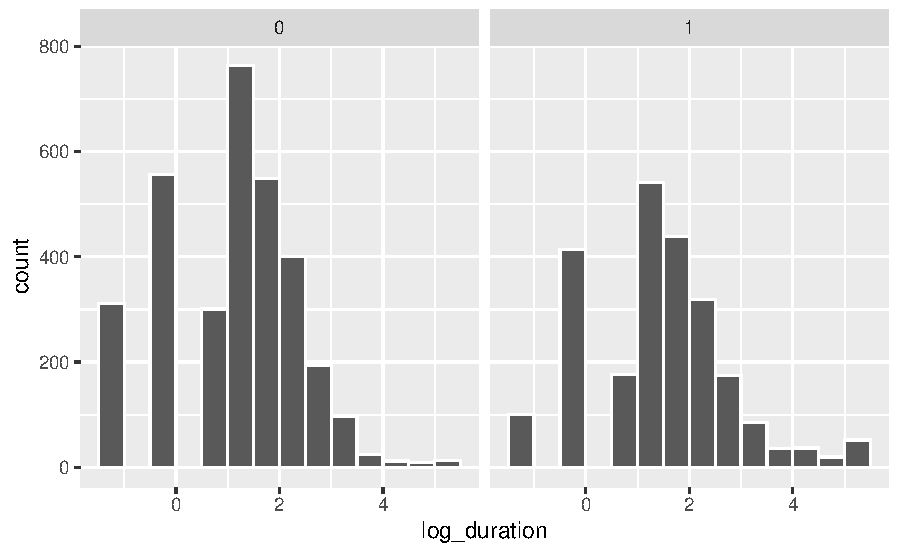
\includegraphics[width=0.75\textwidth,height=\textheight]{DD_wooldridge_injury_files/figure-pdf/log-duration-histogram-1.pdf}

}

\end{figure}

We should also check the distribution of unemployment before and after
the policy change. Copy/paste one of the histogram chunks and change the
faceting:

\begin{Shaded}
\begin{Highlighting}[]
\FunctionTok{ggplot}\NormalTok{(}\AttributeTok{data =}\NormalTok{ injury, }\AttributeTok{mapping =} \FunctionTok{aes}\NormalTok{(}\AttributeTok{x =}\NormalTok{ log\_duration)) }\SpecialCharTok{+}
  \FunctionTok{geom\_histogram}\NormalTok{(}\AttributeTok{binwidth =} \FloatTok{0.5}\NormalTok{, }\AttributeTok{color =} \StringTok{"white"}\NormalTok{, }\AttributeTok{boundary =} \DecValTok{0}\NormalTok{) }\SpecialCharTok{+}
  \FunctionTok{facet\_wrap}\NormalTok{(}\FunctionTok{vars}\NormalTok{(after\_1980))}
\end{Highlighting}
\end{Shaded}

\begin{figure}[H]

{\centering 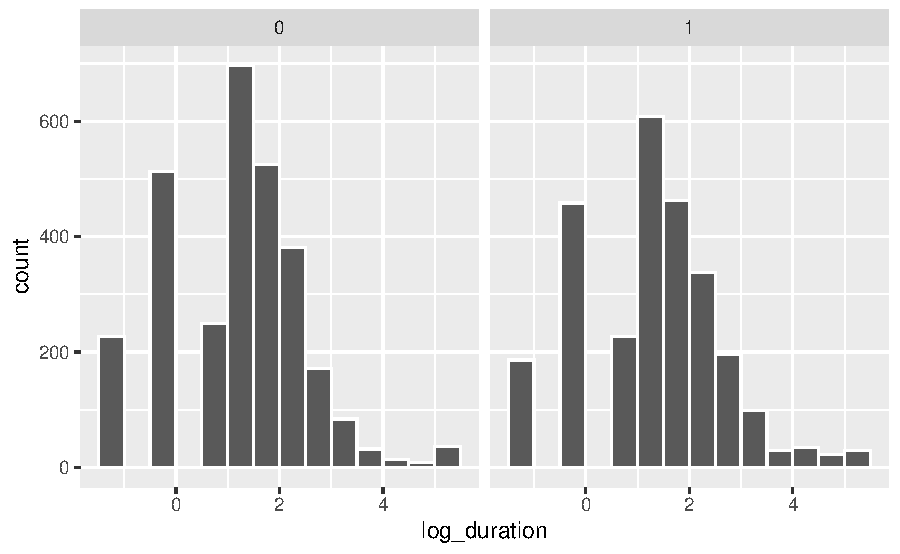
\includegraphics[width=0.75\textwidth,height=\textheight]{DD_wooldridge_injury_files/figure-pdf/log-duration-before-after-histogram-1.pdf}

}

\end{figure}

The distributions look normal-ish, but we can't really easily see
anything different between the before/after and treatment/control
groups. We can plot the averages, though. There are a few different ways
we can do this.

You can use a \texttt{stat\_summary()} layer to have ggplot calculate
summary statistics like averages. Here we just calculate the mean:

\begin{Shaded}
\begin{Highlighting}[]
\FunctionTok{ggplot}\NormalTok{(injury, }\FunctionTok{aes}\NormalTok{(}\AttributeTok{x =} \FunctionTok{factor}\NormalTok{(highearn), }\AttributeTok{y =}\NormalTok{ log\_duration)) }\SpecialCharTok{+}
  \FunctionTok{geom\_point}\NormalTok{(}\AttributeTok{size =} \FloatTok{0.5}\NormalTok{, }\AttributeTok{alpha =} \FloatTok{0.2}\NormalTok{) }\SpecialCharTok{+}
  \FunctionTok{stat\_summary}\NormalTok{(}\AttributeTok{geom =} \StringTok{"point"}\NormalTok{, }\AttributeTok{fun =} \StringTok{"mean"}\NormalTok{, }\AttributeTok{size =} \DecValTok{5}\NormalTok{, }\AttributeTok{color =} \StringTok{"red"}\NormalTok{) }\SpecialCharTok{+}
  \FunctionTok{facet\_wrap}\NormalTok{(}\FunctionTok{vars}\NormalTok{(after\_1980))}
\end{Highlighting}
\end{Shaded}

\begin{figure}[H]

{\centering 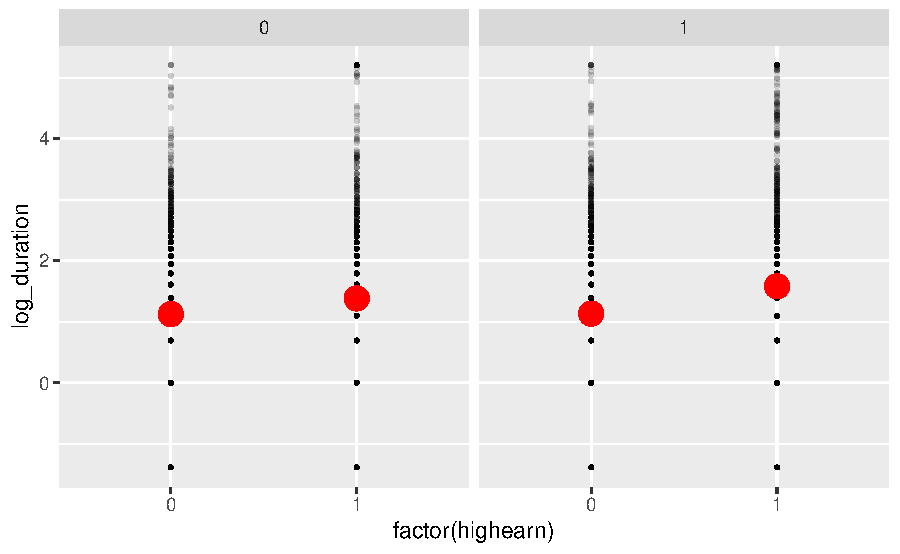
\includegraphics[width=0.75\textwidth,height=\textheight]{DD_wooldridge_injury_files/figure-pdf/plot-means-with-points-1.pdf}

}

\end{figure}

But we can also calculate the mean and 95\% confidence interval:

\begin{Shaded}
\begin{Highlighting}[]
\FunctionTok{ggplot}\NormalTok{(injury, }\FunctionTok{aes}\NormalTok{(}\AttributeTok{x =} \FunctionTok{factor}\NormalTok{(highearn), }\AttributeTok{y =}\NormalTok{ log\_duration)) }\SpecialCharTok{+}
  \FunctionTok{stat\_summary}\NormalTok{(}\AttributeTok{geom =} \StringTok{"pointrange"}\NormalTok{, }\AttributeTok{size =} \DecValTok{1}\NormalTok{, }\AttributeTok{color =} \StringTok{"red"}\NormalTok{,}
               \AttributeTok{fun.data =} \StringTok{"mean\_se"}\NormalTok{, }\AttributeTok{fun.args =} \FunctionTok{list}\NormalTok{(}\AttributeTok{mult =} \FloatTok{1.96}\NormalTok{)) }\SpecialCharTok{+}
  \FunctionTok{facet\_wrap}\NormalTok{(}\FunctionTok{vars}\NormalTok{(after\_1980))}
\end{Highlighting}
\end{Shaded}

\begin{figure}[H]

{\centering 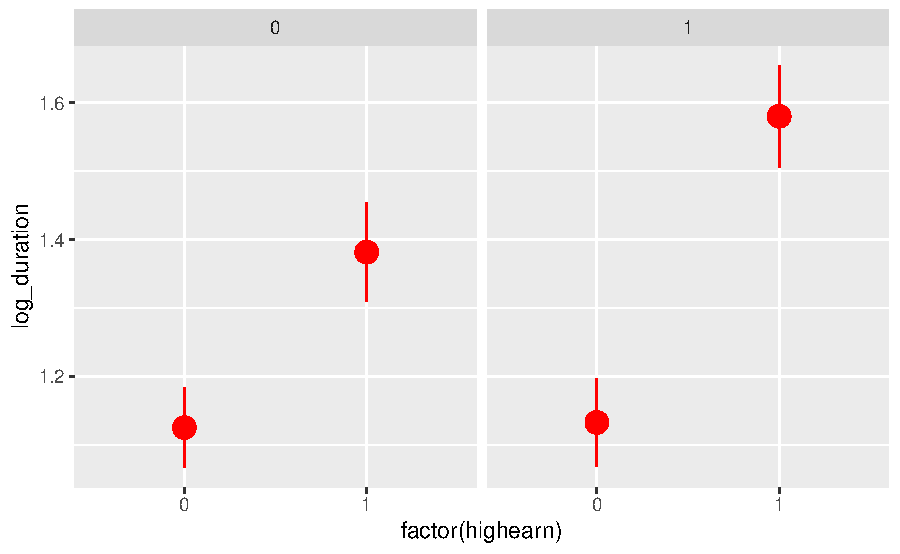
\includegraphics[width=0.75\textwidth,height=\textheight]{DD_wooldridge_injury_files/figure-pdf/plot-means-with-pointrange-1.pdf}

}

\end{figure}

We can already start to see the classical diff-in-diff plot! It looks
like high earners after 1980 had longer unemployment on average.

We can also use \texttt{group\_by()} and \texttt{summarize()} to figure
out group means before sending the data to ggplot. I prefer doing this
because it gives me more control over the data that I'm plotting:

\begin{Shaded}
\begin{Highlighting}[]
\NormalTok{plot\_data }\OtherTok{\textless{}{-}}\NormalTok{ injury }\SpecialCharTok{\%\textgreater{}\%}
  \CommentTok{\# Make these categories instead of 0/1 numbers so they look nicer in the plot}
  \FunctionTok{mutate}\NormalTok{(}\AttributeTok{highearn =} \FunctionTok{factor}\NormalTok{(highearn, }\AttributeTok{labels =} \FunctionTok{c}\NormalTok{(}\StringTok{"Low earner"}\NormalTok{, }\StringTok{"High earner"}\NormalTok{)),}
         \AttributeTok{after\_1980 =} \FunctionTok{factor}\NormalTok{(after\_1980, }\AttributeTok{labels =} \FunctionTok{c}\NormalTok{(}\StringTok{"Before 1980"}\NormalTok{, }\StringTok{"After 1980"}\NormalTok{))) }\SpecialCharTok{\%\textgreater{}\%}
  \FunctionTok{group\_by}\NormalTok{(highearn, after\_1980) }\SpecialCharTok{\%\textgreater{}\%}
  \FunctionTok{summarize}\NormalTok{(}\AttributeTok{mean\_duration =} \FunctionTok{mean}\NormalTok{(log\_duration),}
            \AttributeTok{se\_duration =} \FunctionTok{sd}\NormalTok{(log\_duration) }\SpecialCharTok{/} \FunctionTok{sqrt}\NormalTok{(}\FunctionTok{n}\NormalTok{()),}
            \AttributeTok{upper =}\NormalTok{ mean\_duration }\SpecialCharTok{+}\NormalTok{ (}\FloatTok{1.96} \SpecialCharTok{*}\NormalTok{ se\_duration),}
            \AttributeTok{lower =}\NormalTok{ mean\_duration }\SpecialCharTok{+}\NormalTok{ (}\SpecialCharTok{{-}}\FloatTok{1.96} \SpecialCharTok{*}\NormalTok{ se\_duration))}

\FunctionTok{ggplot}\NormalTok{(plot\_data, }\FunctionTok{aes}\NormalTok{(}\AttributeTok{x =}\NormalTok{ highearn, }\AttributeTok{y =}\NormalTok{ mean\_duration)) }\SpecialCharTok{+}
  \FunctionTok{geom\_pointrange}\NormalTok{(}\FunctionTok{aes}\NormalTok{(}\AttributeTok{ymin =}\NormalTok{ lower, }\AttributeTok{ymax =}\NormalTok{ upper),}
                  \AttributeTok{color =} \StringTok{"darkgreen"}\NormalTok{, }\AttributeTok{size =} \DecValTok{1}\NormalTok{) }\SpecialCharTok{+}
  \FunctionTok{facet\_wrap}\NormalTok{(}\FunctionTok{vars}\NormalTok{(after\_1980))}
\end{Highlighting}
\end{Shaded}

\begin{figure}[H]

{\centering 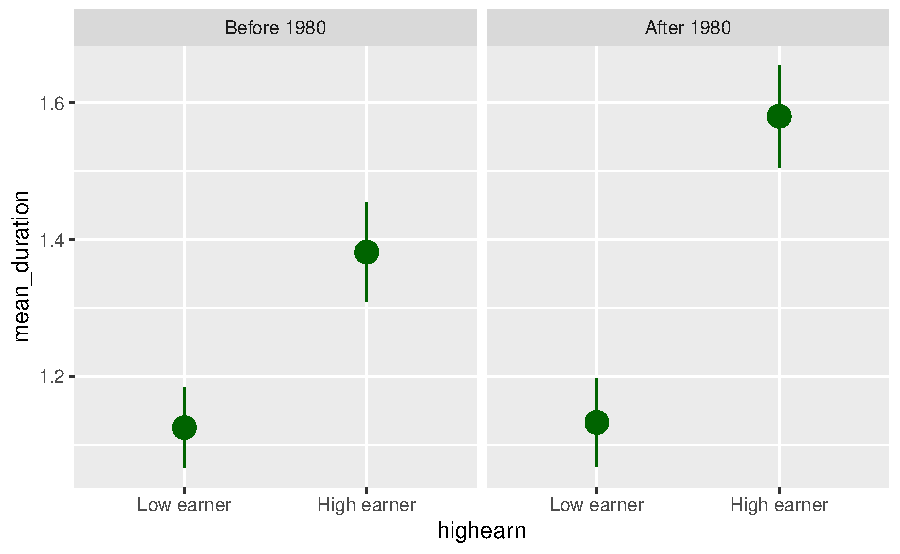
\includegraphics[width=0.75\textwidth,height=\textheight]{DD_wooldridge_injury_files/figure-pdf/plot-pointrange-manual-1.pdf}

}

\end{figure}

Or, plotted in the more standard diff-in-diff format:

\begin{Shaded}
\begin{Highlighting}[]
\FunctionTok{ggplot}\NormalTok{(plot\_data, }\FunctionTok{aes}\NormalTok{(}\AttributeTok{x =}\NormalTok{ after\_1980, }\AttributeTok{y =}\NormalTok{ mean\_duration, }\AttributeTok{color =}\NormalTok{ highearn)) }\SpecialCharTok{+}
  \FunctionTok{geom\_pointrange}\NormalTok{(}\FunctionTok{aes}\NormalTok{(}\AttributeTok{ymin =}\NormalTok{ lower, }\AttributeTok{ymax =}\NormalTok{ upper), }\AttributeTok{size =} \DecValTok{1}\NormalTok{) }\SpecialCharTok{+}
  \CommentTok{\# The group = highearn here makes it so the lines go across categories}
  \FunctionTok{geom\_line}\NormalTok{(}\FunctionTok{aes}\NormalTok{(}\AttributeTok{group =}\NormalTok{ highearn))}
\end{Highlighting}
\end{Shaded}

\begin{figure}[H]

{\centering 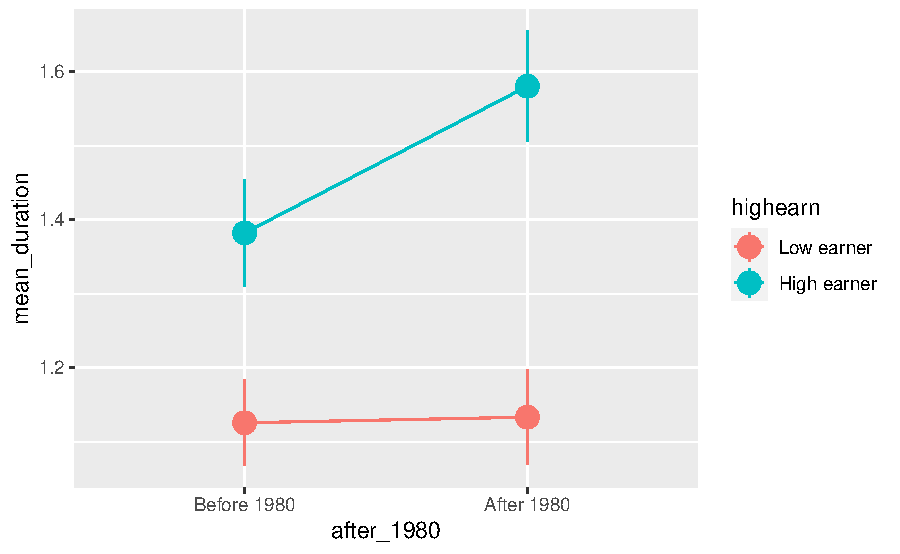
\includegraphics[width=0.75\textwidth,height=\textheight]{DD_wooldridge_injury_files/figure-pdf/plot-pointrange-manual-no-facet-1.pdf}

}

\end{figure}

\hypertarget{diff-in-diff-by-hand}{%
\subsection{Diff-in-diff by hand}\label{diff-in-diff-by-hand}}

We can find that exact difference by filling out the 2x2 before/after
treatment/control table:

\begin{longtable}[]{@{}lccc@{}}
\toprule()
& Before 1980 & After 1980 & ∆ \\
\midrule()
\endhead
Low earners & A & B & B − A \\
High earners & C & D & D − C \\
∆ & C − A & D − B & (D − C) − (B − A) \\
\bottomrule()
\end{longtable}

A combination of \texttt{group\_by()} and \texttt{summarize()} makes
this really easy:

\begin{Shaded}
\begin{Highlighting}[]
\NormalTok{diffs }\OtherTok{\textless{}{-}}\NormalTok{ injury }\SpecialCharTok{\%\textgreater{}\%}
  \FunctionTok{group\_by}\NormalTok{(after\_1980, highearn) }\SpecialCharTok{\%\textgreater{}\%}
  \FunctionTok{summarize}\NormalTok{(}\AttributeTok{mean\_duration =} \FunctionTok{mean}\NormalTok{(log\_duration),}
            \CommentTok{\# Calculate average with regular duration too, just for fun}
            \AttributeTok{mean\_duration\_for\_humans =} \FunctionTok{mean}\NormalTok{(duration))}
\NormalTok{diffs}
\DocumentationTok{\#\# \# A tibble: 4 x 4}
\DocumentationTok{\#\# \# Groups:   after\_1980 [2]}
\DocumentationTok{\#\#   after\_1980 highearn mean\_duration mean\_duration\_for\_humans}
\DocumentationTok{\#\#        \textless{}dbl\textgreater{}    \textless{}dbl\textgreater{}         \textless{}dbl\textgreater{}                    \textless{}dbl\textgreater{}}
\DocumentationTok{\#\# 1          0        0          1.13                     6.27}
\DocumentationTok{\#\# 2          0        1          1.38                    11.2 }
\DocumentationTok{\#\# 3          1        0          1.13                     7.04}
\DocumentationTok{\#\# 4          1        1          1.58                    12.9}
\end{Highlighting}
\end{Shaded}

We can pull each of these numbers out of the table with some
\texttt{filter()}s and \texttt{pull()}:

\begin{Shaded}
\begin{Highlighting}[]
\NormalTok{before\_treatment }\OtherTok{\textless{}{-}}\NormalTok{ diffs }\SpecialCharTok{\%\textgreater{}\%}
  \FunctionTok{filter}\NormalTok{(after\_1980 }\SpecialCharTok{==} \DecValTok{0}\NormalTok{, highearn }\SpecialCharTok{==} \DecValTok{1}\NormalTok{) }\SpecialCharTok{\%\textgreater{}\%}
  \FunctionTok{pull}\NormalTok{(mean\_duration)}

\NormalTok{before\_control }\OtherTok{\textless{}{-}}\NormalTok{ diffs }\SpecialCharTok{\%\textgreater{}\%}
  \FunctionTok{filter}\NormalTok{(after\_1980 }\SpecialCharTok{==} \DecValTok{0}\NormalTok{, highearn }\SpecialCharTok{==} \DecValTok{0}\NormalTok{) }\SpecialCharTok{\%\textgreater{}\%}
  \FunctionTok{pull}\NormalTok{(mean\_duration)}

\NormalTok{after\_treatment }\OtherTok{\textless{}{-}}\NormalTok{ diffs }\SpecialCharTok{\%\textgreater{}\%}
  \FunctionTok{filter}\NormalTok{(after\_1980 }\SpecialCharTok{==} \DecValTok{1}\NormalTok{, highearn }\SpecialCharTok{==} \DecValTok{1}\NormalTok{) }\SpecialCharTok{\%\textgreater{}\%}
  \FunctionTok{pull}\NormalTok{(mean\_duration)}

\NormalTok{after\_control }\OtherTok{\textless{}{-}}\NormalTok{ diffs }\SpecialCharTok{\%\textgreater{}\%}
  \FunctionTok{filter}\NormalTok{(after\_1980 }\SpecialCharTok{==} \DecValTok{1}\NormalTok{, highearn }\SpecialCharTok{==} \DecValTok{0}\NormalTok{) }\SpecialCharTok{\%\textgreater{}\%}
  \FunctionTok{pull}\NormalTok{(mean\_duration)}

\NormalTok{diff\_treatment\_before\_after }\OtherTok{\textless{}{-}}\NormalTok{ after\_treatment }\SpecialCharTok{{-}}\NormalTok{ before\_treatment}
\NormalTok{diff\_treatment\_before\_after}
\DocumentationTok{\#\# [1] 0.2}

\NormalTok{diff\_control\_before\_after }\OtherTok{\textless{}{-}}\NormalTok{ after\_control }\SpecialCharTok{{-}}\NormalTok{ before\_control}
\NormalTok{diff\_control\_before\_after}
\DocumentationTok{\#\# [1] 0.0077}

\NormalTok{diff\_diff }\OtherTok{\textless{}{-}}\NormalTok{ diff\_treatment\_before\_after }\SpecialCharTok{{-}}\NormalTok{ diff\_control\_before\_after}
\NormalTok{diff\_diff}
\DocumentationTok{\#\# [1] 0.19}
\end{Highlighting}
\end{Shaded}

The diff-in-diff estimate is 0.19, which means that the program causes
an increase in unemployment duration of 0.19 logged weeks. Logged weeks
is nonsensical, though, so we have to interpret it with percentages
(\href{https://stats.stackexchange.com/a/18639/3025}{here's a handy
guide!}; this is Example B, where the dependent/outcome variable is
logged). Receiving the treatment (i.e.~being a high earner after the
change in policy) causes a 19\% increase in the length of unemployment.

\begin{Shaded}
\begin{Highlighting}[]
\FunctionTok{ggplot}\NormalTok{(diffs, }\FunctionTok{aes}\NormalTok{(}\AttributeTok{x =} \FunctionTok{as.factor}\NormalTok{(after\_1980),}
                  \AttributeTok{y =}\NormalTok{ mean\_duration,}
                  \AttributeTok{color =} \FunctionTok{as.factor}\NormalTok{(highearn))) }\SpecialCharTok{+}
  \FunctionTok{geom\_point}\NormalTok{() }\SpecialCharTok{+}
  \FunctionTok{geom\_line}\NormalTok{(}\FunctionTok{aes}\NormalTok{(}\AttributeTok{group =} \FunctionTok{as.factor}\NormalTok{(highearn))) }\SpecialCharTok{+}
  \CommentTok{\# If you use these lines you\textquotesingle{}ll get some extra annotation lines and}
  \CommentTok{\# labels. The annotate() function lets you put stuff on a ggplot that\textquotesingle{}s not}
  \CommentTok{\# part of a dataset. Normally with geom\_line, geom\_point, etc., you have to}
  \CommentTok{\# plot data that is in columns. With annotate() you can specify your own x and}
  \CommentTok{\# y values.}
  \FunctionTok{annotate}\NormalTok{(}\AttributeTok{geom =} \StringTok{"segment"}\NormalTok{, }\AttributeTok{x =} \StringTok{"0"}\NormalTok{, }\AttributeTok{xend =} \StringTok{"1"}\NormalTok{,}
           \AttributeTok{y =}\NormalTok{ before\_treatment, }\AttributeTok{yend =}\NormalTok{ after\_treatment }\SpecialCharTok{{-}}\NormalTok{ diff\_diff,}
           \AttributeTok{linetype =} \StringTok{"dashed"}\NormalTok{, }\AttributeTok{color =} \StringTok{"grey50"}\NormalTok{) }\SpecialCharTok{+}
  \FunctionTok{annotate}\NormalTok{(}\AttributeTok{geom =} \StringTok{"segment"}\NormalTok{, }\AttributeTok{x =} \StringTok{"1"}\NormalTok{, }\AttributeTok{xend =} \StringTok{"1"}\NormalTok{,}
           \AttributeTok{y =}\NormalTok{ after\_treatment, }\AttributeTok{yend =}\NormalTok{ after\_treatment }\SpecialCharTok{{-}}\NormalTok{ diff\_diff,}
           \AttributeTok{linetype =} \StringTok{"dotted"}\NormalTok{, }\AttributeTok{color =} \StringTok{"blue"}\NormalTok{) }\SpecialCharTok{+}
  \FunctionTok{annotate}\NormalTok{(}\AttributeTok{geom =} \StringTok{"label"}\NormalTok{, }\AttributeTok{x =} \StringTok{"1"}\NormalTok{, }\AttributeTok{y =}\NormalTok{ after\_treatment }\SpecialCharTok{{-}}\NormalTok{ (diff\_diff }\SpecialCharTok{/} \DecValTok{2}\NormalTok{),}
           \AttributeTok{label =} \StringTok{"Program effect"}\NormalTok{, }\AttributeTok{size =} \DecValTok{3}\NormalTok{)}
\end{Highlighting}
\end{Shaded}

\begin{figure}[H]

{\centering 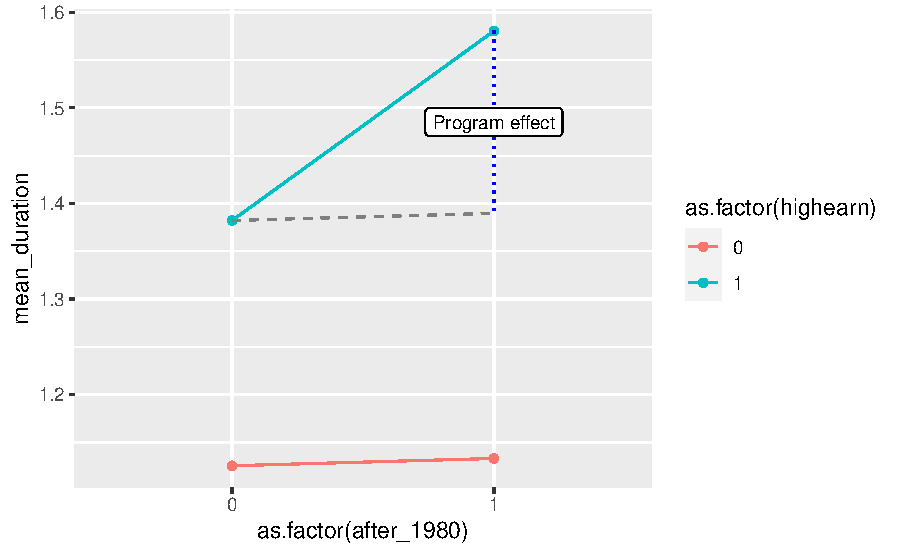
\includegraphics[width=0.75\textwidth,height=\textheight]{DD_wooldridge_injury_files/figure-pdf/nice-diff-diff-plot-1.pdf}

}

\end{figure}

\begin{Shaded}
\begin{Highlighting}[]

\CommentTok{\# Here, all the as.factor changes are directly in the ggplot code. I generally}
\CommentTok{\# don\textquotesingle{}t like doing this and prefer to do that separately so there\textquotesingle{}s less typing}
\CommentTok{\# in the ggplot code, like this:}
\CommentTok{\#}
\CommentTok{\# diffs \textless{}{-} diffs \%\textgreater{}\%}
\CommentTok{\#   mutate(after\_1980 = as.factor(after\_1980), highearn = as.factor(highearn))}
\CommentTok{\#}
\CommentTok{\# ggplot(diffs, aes(x = after\_1980, y = avg\_durat, color = highearn)) +}
\CommentTok{\#   geom\_line(aes(group = highearn))}
\end{Highlighting}
\end{Shaded}

\hypertarget{diff-in-diff-with-regression}{%
\subsection{Diff-in-diff with
regression}\label{diff-in-diff-with-regression}}

Calculating all the pieces by hand like that is tedious, so we can use
regression to do it instead! Remember that we need to include indicator
variables for treatment/control and for before/after, as well as the
interaction of the two. Here's what the math equation looks like:

\[
\begin{aligned}
\log(\text{duration}) = &\alpha + \beta \ \text{highearn} + \gamma \ \text{after_1980} + \\
& \delta \ (\text{highearn} \times \text{after_1980}) + \epsilon
\end{aligned}
\]

The \(\delta\) coefficient is the effect we care about in the
end---that's the diff-in-diff estimator.

\begin{Shaded}
\begin{Highlighting}[]
\NormalTok{model\_small }\OtherTok{\textless{}{-}} \FunctionTok{lm}\NormalTok{(log\_duration }\SpecialCharTok{\textasciitilde{}}\NormalTok{ highearn }\SpecialCharTok{+}\NormalTok{ after\_1980 }\SpecialCharTok{+}\NormalTok{ highearn }\SpecialCharTok{*}\NormalTok{ after\_1980,}
                  \AttributeTok{data =}\NormalTok{ injury)}
\FunctionTok{tidy}\NormalTok{(model\_small)}
\DocumentationTok{\#\# \# A tibble: 4 x 5}
\DocumentationTok{\#\#   term                estimate std.error statistic   p.value}
\DocumentationTok{\#\#   \textless{}chr\textgreater{}                  \textless{}dbl\textgreater{}     \textless{}dbl\textgreater{}     \textless{}dbl\textgreater{}     \textless{}dbl\textgreater{}}
\DocumentationTok{\#\# 1 (Intercept)          1.13       0.0307    36.6   1.62e{-}263}
\DocumentationTok{\#\# 2 highearn             0.256      0.0474     5.41  6.72e{-}  8}
\DocumentationTok{\#\# 3 after\_1980           0.00766    0.0447     0.171 8.64e{-}  1}
\DocumentationTok{\#\# 4 highearn:after\_1980  0.191      0.0685     2.78  5.42e{-}  3}
\end{Highlighting}
\end{Shaded}

The coefficient for \texttt{highearn:after\_1980} is the same as what we
found by hand, as it should be! It is statistically significant, so we
can be fairly confident that it is not 0.

\hypertarget{diff-in-diff-with-regression-controls}{%
\subsection{Diff-in-diff with regression +
controls}\label{diff-in-diff-with-regression-controls}}

One advantage to using regression for diff-in-diff is that we can
include control variables to help isolate the effect. For example,
perhaps claims made by construction or manufacturing workers tend to
have longer duration than claims made workers in other industries. Or
maybe those claiming back injuries tend to have longer claims than those
claiming head injuries. We might also want to control for worker
demographics such as gender, marital status, and age.

Let's estimate an expanded version of the basic regression model with
the following additional variables:

\begin{itemize}
\tightlist
\item
  \texttt{male}
\item
  \texttt{married}
\item
  \texttt{age}
\item
  \texttt{hosp} (1 = hospitalized)
\item
  \texttt{indust} (1 = manuf, 2 = construc, 3 = other)
\item
  \texttt{injtype} (1-8; categories for different types of injury)
\item
  \texttt{lprewage} (log of wage prior to filing a claim)
\end{itemize}

\emph{Important}: \texttt{indust} and \texttt{injtype} are in the
dataset as numbers (1-3 and 1-8), but they're actually categories. We
have to tell R to treat them as categories (or factors), otherwise it'll
assume that you can have an injury type of 3.46 or something impossible.

\begin{Shaded}
\begin{Highlighting}[]
\CommentTok{\# Convert industry and injury type to categories/factors}
\NormalTok{injury\_fixed }\OtherTok{\textless{}{-}}\NormalTok{ injury }\SpecialCharTok{\%\textgreater{}\%}
  \FunctionTok{mutate}\NormalTok{(}\AttributeTok{indust =} \FunctionTok{as.factor}\NormalTok{(indust),}
         \AttributeTok{injtype =} \FunctionTok{as.factor}\NormalTok{(injtype))}
\end{Highlighting}
\end{Shaded}

\begin{Shaded}
\begin{Highlighting}[]
\NormalTok{model\_big }\OtherTok{\textless{}{-}} \FunctionTok{lm}\NormalTok{(log\_duration }\SpecialCharTok{\textasciitilde{}}\NormalTok{ highearn }\SpecialCharTok{+}\NormalTok{ after\_1980 }\SpecialCharTok{+}\NormalTok{ highearn }\SpecialCharTok{*}\NormalTok{ after\_1980 }\SpecialCharTok{+}
\NormalTok{                  male }\SpecialCharTok{+}\NormalTok{ married }\SpecialCharTok{+}\NormalTok{ age }\SpecialCharTok{+}\NormalTok{ hosp }\SpecialCharTok{+}\NormalTok{ indust }\SpecialCharTok{+}\NormalTok{ injtype }\SpecialCharTok{+}\NormalTok{ lprewage,}
                \AttributeTok{data =}\NormalTok{ injury\_fixed)}
\FunctionTok{tidy}\NormalTok{(model\_big)}
\DocumentationTok{\#\# \# A tibble: 18 x 5}
\DocumentationTok{\#\#    term                estimate std.error statistic   p.value}
\DocumentationTok{\#\#    \textless{}chr\textgreater{}                  \textless{}dbl\textgreater{}     \textless{}dbl\textgreater{}     \textless{}dbl\textgreater{}     \textless{}dbl\textgreater{}}
\DocumentationTok{\#\#  1 (Intercept)         {-}1.53      0.422       {-}3.62 2.98e{-}  4}
\DocumentationTok{\#\#  2 highearn            {-}0.152     0.0891      {-}1.70 8.86e{-}  2}
\DocumentationTok{\#\#  3 after\_1980           0.0495    0.0413       1.20 2.31e{-}  1}
\DocumentationTok{\#\#  4 male                {-}0.0843    0.0423      {-}1.99 4.64e{-}  2}
\DocumentationTok{\#\#  5 married              0.0567    0.0373       1.52 1.29e{-}  1}
\DocumentationTok{\#\#  6 age                  0.00651   0.00134      4.86 1.19e{-}  6}
\DocumentationTok{\#\#  7 hosp                 1.13      0.0370      30.5  5.20e{-}189}
\DocumentationTok{\#\#  8 indust2              0.184     0.0541       3.40 6.87e{-}  4}
\DocumentationTok{\#\#  9 indust3              0.163     0.0379       4.32 1.60e{-}  5}
\DocumentationTok{\#\# 10 injtype2             0.935     0.144        6.51 8.29e{-} 11}
\DocumentationTok{\#\# 11 injtype3             0.635     0.0854       7.44 1.19e{-} 13}
\DocumentationTok{\#\# 12 injtype4             0.555     0.0928       5.97 2.49e{-}  9}
\DocumentationTok{\#\# 13 injtype5             0.641     0.0854       7.51 7.15e{-} 14}
\DocumentationTok{\#\# 14 injtype6             0.615     0.0863       7.13 1.17e{-} 12}
\DocumentationTok{\#\# 15 injtype7             0.991     0.191        5.20 2.03e{-}  7}
\DocumentationTok{\#\# 16 injtype8             0.434     0.119        3.65 2.64e{-}  4}
\DocumentationTok{\#\# 17 lprewage             0.284     0.0801       3.55 3.83e{-}  4}
\DocumentationTok{\#\# 18 highearn:after\_1980  0.169     0.0640       2.64 8.38e{-}  3}

\CommentTok{\# Extract just the diff{-}in{-}diff estimate}
\NormalTok{diff\_diff\_controls }\OtherTok{\textless{}{-}} \FunctionTok{tidy}\NormalTok{(model\_big) }\SpecialCharTok{\%\textgreater{}\%}
  \FunctionTok{filter}\NormalTok{(term }\SpecialCharTok{==} \StringTok{"highearn:after\_1980"}\NormalTok{) }\SpecialCharTok{\%\textgreater{}\%}
  \FunctionTok{pull}\NormalTok{(estimate)}
\end{Highlighting}
\end{Shaded}

After controlling for a host of demographic controls, the diff-in-diff
estimate is smaller (0.17), indicating that the policy caused a 17\%
increase in the duration of weeks unemployed following a workplace
injury. It is smaller because the other independent variables now
explain some of the variation in \texttt{log\_duration}.

\hypertarget{comparison-of-results}{%
\subsection{Comparison of results}\label{comparison-of-results}}

We can put the model coefficients side-by-side to compare the value for
\texttt{highearn:after\_1980} as we change the model.

\begin{Shaded}
\begin{Highlighting}[]
\FunctionTok{modelsummary}\NormalTok{(}\FunctionTok{list}\NormalTok{(}\StringTok{"Simple"} \OtherTok{=}\NormalTok{ model\_small, }\StringTok{"Full"} \OtherTok{=}\NormalTok{ model\_big))}
\end{Highlighting}
\end{Shaded}

\begin{table}
\centering
\begin{tabular}[t]{lcc}
\toprule
  & Simple & Full\\
\midrule
(Intercept) & \num{1.126}*** & \num{-1.528}***\\
 & (\num{0.031}) & (\num{0.422})\\
highearn & \num{0.256}*** & \num{-0.152}+\\
 & (\num{0.047}) & (\num{0.089})\\
after\_1980 & \num{0.008} & \num{0.050}\\
 & (\num{0.045}) & (\num{0.041})\\
\cellcolor[HTML]{F6D645}{highearn × after\_1980} & \cellcolor[HTML]{F6D645}{\num{0.191}**} & \cellcolor[HTML]{F6D645}{\num{0.169}**}\\
 & (\num{0.069}) & (\num{0.064})\\
male &  & \num{-0.084}*\\
 &  & (\num{0.042})\\
married &  & \num{0.057}\\
 &  & \vphantom{1} (\num{0.037})\\
age &  & \num{0.007}***\\
 &  & (\num{0.001})\\
hosp &  & \num{1.130}***\\
 &  & (\num{0.037})\\
indust2 &  & \num{0.184}***\\
 &  & (\num{0.054})\\
indust3 &  & \num{0.163}***\\
 &  & (\num{0.038})\\
injtype2 &  & \num{0.935}***\\
 &  & (\num{0.144})\\
injtype3 &  & \num{0.635}***\\
 &  & \vphantom{1} (\num{0.085})\\
injtype4 &  & \num{0.555}***\\
 &  & (\num{0.093})\\
injtype5 &  & \num{0.641}***\\
 &  & (\num{0.085})\\
injtype6 &  & \num{0.615}***\\
 &  & (\num{0.086})\\
injtype7 &  & \num{0.991}***\\
 &  & (\num{0.191})\\
injtype8 &  & \num{0.434}***\\
 &  & (\num{0.119})\\
lprewage &  & \num{0.284}***\\
 &  & (\num{0.080})\\
\midrule
Num.Obs. & \num{5626} & \num{5347}\\
R2 & \num{0.021} & \num{0.190}\\
R2 Adj. & \num{0.020} & \num{0.187}\\
\bottomrule
\multicolumn{3}{l}{\rule{0pt}{1em}+ p $<$ 0.1, * p $<$ 0.05, ** p $<$ 0.01, *** p $<$ 0.001}\\
\end{tabular}
\end{table}



\end{document}
